% !TEX root = ../master.tex
\chapter{Fundamentals}
\label{chap:sota}

\section{Computer Vision}

TODO

\ref{fig:sota:imageengineering}
\begin{figure}[hbt]
	\centering
	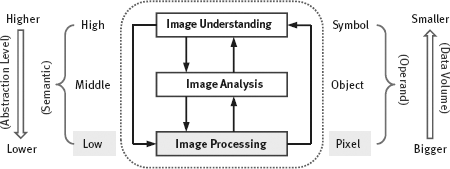
\includegraphics[width=0.8\textwidth, keepaspectratio]{08_Chapter01_fig1-4}
	\caption[]{\label{fig:sota:imageengineering} TODO Caption
	Reprinted from \textcite[][Chapter~1]{zhang2017imageprocessing}}
\end{figure}

\subsection{Object Detection}

TODO
edge detection, outline detection
foreground background mask from video image
background substraction

\subsection{Volume Estimation}

TODO
single view, multiview, depth sensors
estimation by pixel area
interpolation of depth information by combinding views
bounding / section box
full 3d reconstruction
\ref{fig:sota:mulitviewtop}

\begin{figure}[hbt]
	\centering
	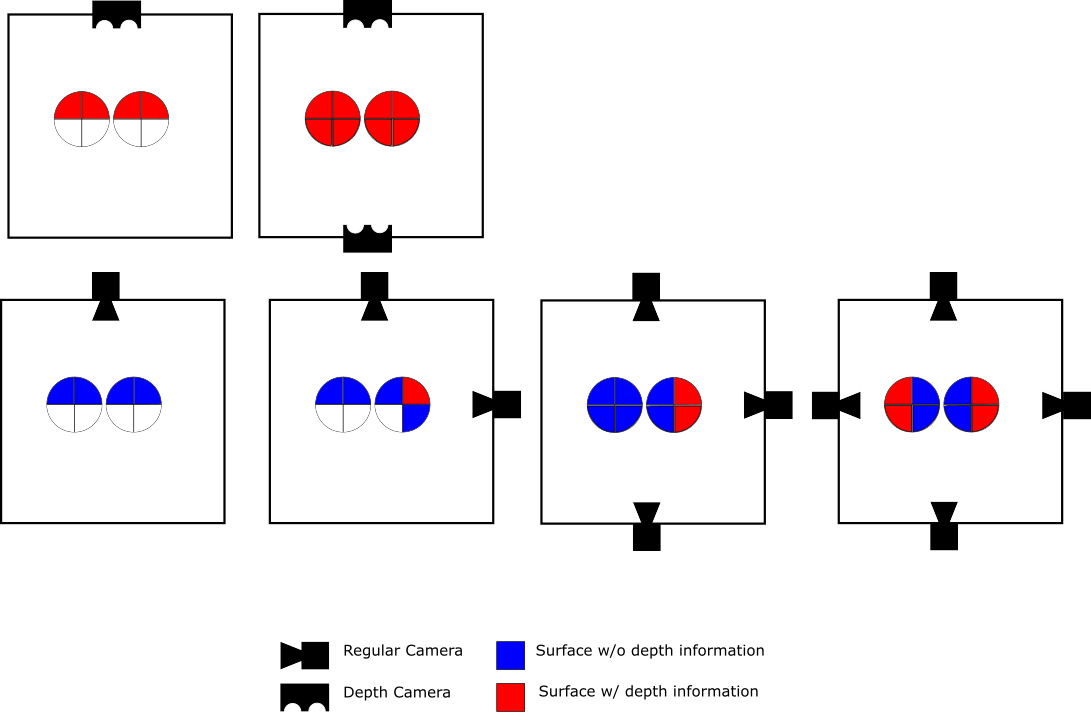
\includegraphics[width=1.0\textwidth, keepaspectratio]{resources/multiview}
	\caption[]{\label{fig:sota:mulitviewtop}TODO Caption
	Based on and adapted from \textcite[][]{sonaten2011volume}}
\end{figure}


\section{Elevator Control}
TODO shor introtuction, definition and what are important aspects about it

\subsection{System Components}
TODO
- shaft and movement mechanism
- motors
- car / cabin / convoyance
- doors
- in cabing panel
- panel on each floor
- advanced cabin sensory
- advanced floor sensory
- control electronic per elevator
-- motor control (cabin dispatch)
-- door control
-- security system
- grou controller
TODO find picture or reference
\ref{fig:sota:groupcontroller}

\begin{figure}[hbt]
	\centering
	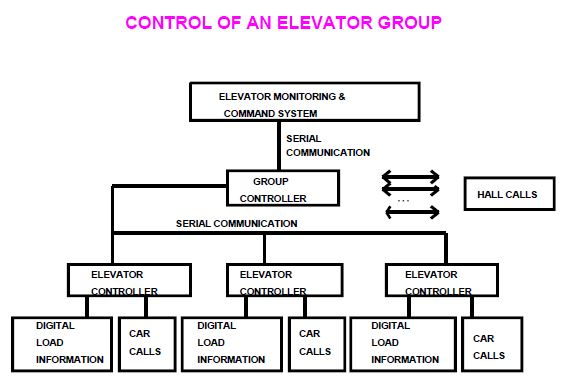
\includegraphics[width=1.0\textwidth, keepaspectratio]{resources/group_controller}
	\caption[]{\label{fig:sota:groupcontroller} TODO Caption
	Reprinted from \textcite[][p.~10]{siikonen1997models}}
\end{figure}



\subsection{System Classifications}
TODO
- by amount of elevators
- by type of sensory to haul the car
TODO how many elevators parallel
TODO additional travel information: how many people inside and outside, up / down / floor select inside / outside, everyone presses?, video? 
destination control system
- type of goods / people transported \autocite[][p.~141]{unger2015aufzuege}

\subsection{Passenger Flow Patterns}
TODO
TODO time of day eg. upstream, down stream, cross stream

\autocite[][pp.~1--2]{beers2015arrivals}
\autocite[][pp.~6--7]{axelsson2013strategies}
\autocite[][p.~194]{unger2015aufzuege}

\subsection{Control Strategies}
TODO

\autocite[][pp.~3--4,10]{beers2015arrivals}
- stopping policies / strategies
- parking polcies
- call allocation

\autocite[][pp.~3--6]{axelsson2013strategies}
- collective control
- zoneing
- search based
- rule based
- genetic algorithm




\subsection{Performance Criteria}
TODO
criteria: waiting time for passengers, riding time for passengers, total journey time, capacity utilization (average and maximal), energy consumption, roundtriptime, total number of stops
ca 80\% oder auch 60-70\% maximal load on car, could be lower if objects in it
space vs wheight utilization
riding comfort in space and speed

\autocite[][p.~10]{beers2015arrivals}


\subsection{Simulational Optimization Approaches}
TODO
model building etc: here is a lot of research in the topic utilizing theoretical multivariable model optimization, simulational approaches and heuristical approaches in real world (refs?)

\autocite[][pp.~7--11]{beers2015arrivals}
\autocite[][p.~193]{unger2015aufzuege}


TODO
